\documentclass[a4paper,12pt,oneside]{book}

%------------------------------- Start of the Preable ------------------------------------------------
\usepackage[english]{babel}
\addto{\captionsenglish}{%
\renewcommand{\bibname}{References}
\renewcommand{\refname}{References}
}

\usepackage{blindtext}
\usepackage{minted}
\setcounter{secnumdepth}{3}

%\usepackage[none]{hyphenat}
\usepackage[parfill]{parskip}

\usepackage{hyperref}
\hypersetup{
    colorlinks=true,
    linkcolor=blue,
    filecolor=magenta,      
    urlcolor=cyan,
}

\urlstyle{same}
%use of package fancy header
\usepackage{fancyhdr}
\usepackage{fancyvrb}
\setlength\headheight{26pt}
\fancyhf{}
%\rhead{
\includegraphics[width=1cm]{logo}}
\lhead{\rightmark}
\rhead{
\includegraphics[width=1cm]{images/logo}}
\fancyfoot[RE, RO]{\thepage}
\fancyfoot[CE, CO]{\href{http://www.e-yantra.org}{www.e-yantra.org}}

\pagestyle{fancy}

%use of package for section title formatting
\usepackage{titlesec}
\titleformat{\chapter}
  {\Large\bfseries} % format
  {}                % label
  {0pt}             % sep
  {\huge}           % before-code
 
%use of package tcolorbox for colorful textbox
\usepackage[most]{tcolorbox}
\tcbset{colback=cyan!5!white,colframe=cyan!75!black,halign title = flush center}

\newtcolorbox{mybox}[1]{colback=cyan!5!white,
colframe=cyan!75!black,fonttitle=\bfseries,
title=\textbf{\Large{#1}}}

%use of package marginnote for notes in margin
\usepackage{marginnote}

%use of packgage watermark for pages
%\usepackage{draftwatermark}
%\SetWatermarkText{
\includegraphics{logo}}
\usepackage[scale=3.2,opacity=0.1,angle=0]{background}
\backgroundsetup{
contents={
\includegraphics{images/logo-med}}
}

%use of newcommand for keywords color
\usepackage{xcolor}
\newcommand{\keyword}[1]{\textcolor{red}{\textbf{#1}}}

%package for inserting pictures
\usepackage{graphicx}

%package for highlighting
\usepackage{color,soul}

%new command for table
\newcommand{\head}[1]{\textnormal{\textbf{#1}}}

\usepackage{dirtree}
\usepackage{siunitx}

\makeatletter
\global\let\tikz@ensure@dollar@catcode=\relax
\makeatother

\usepackage{textcomp}

%---------------------- End of the Preamble ---------------------------------------


\begin{document}

%---------------------Title Page------------------------------------------------
\begin{titlepage}
\raggedright
{\Large eYSIP 2017\\[1cm]}
{\Huge \scshape Tutorial on MultiWii Serial Protocol \\[.1in]}

\vfill

\begin{figure}[!htb]
\centering

\includegraphics[width=0.7\textwidth]{images/multiwii}
\end{figure}

\vfill

\begin{flushright}
{\large Heethesh Vhavle \\}
{\large Sanam Shakya \\}
{\large Pushkar Raj \\}
\vspace{0.5cm}
{\large Duration of Internship: $ 22/05/2017-07/07/2017 $ \\}
\end{flushright}
\medskip

{\itshape 2017, e-Yantra Publication}
\end{titlepage}

%-------------------------------------------------------------------------------

%\tableofcontents
%\listoffigures

%-------------------------------------------------------------------------------

\chapter[MultiWii Serial Protocol]{MultiWii Serial Protocol}
\section{Introduction}
The project deals with the study of control algorithms and to develop a custom firmware for quadcopter (flight controller) on 32-bit micro-controllers such as the STM32F1xx (ARM® Cortex®-M3 core). The flight controller is designed to control parameters such as the throttle, yaw, pitch and roll and consists of algorithms considering various motion and dynamics. Another goal is to develop a wireless joystick controller for simple maneuvering of the quadcopter.\\

Fine tuning PID values of a quadcopter flight controller can be very devious and time consuming process if a programmer needs to adjust parameters in source code, compile it and upload the new program to copter every time they want to make a slight adjustment.\\ 

In addition to transferring new PID values to quadcopter, we can also request other data from the quadcopter, such as current PID values, sensor readings, flight status, motor values and any other data useful in error handling, debugging or even visualization.\\

A trivial problem that follows this is a standard and a secure method of data transfer. There has to some method to differentiate the various data types that we require to transmit. The \textit{MultiWii Serial Protocol (MSP)} has been devised to solve this exact problem.\\

\clearpage

\section{MultiWii Serial Protocol}
\textit{MultiWii Serial Protocol} is a part of the MultiWii flight controller firmware and has gained popularity and is currently widely used as the communication protocol in many flight controllers. It is a standard, secure and light weight protocol. MSP operates over UART communication. The data to be sent or received is packed into a frame. Each frame has a header, data payload and a checksum. The frame format is explained in detail below.\\

\textbf{Header} | Every frame begins with the characters \textit{'\$'} followed \textit{'M'}. The next element represents the direction of the data transfer. '$<$' indicates that the data is being sent to the quadcopter and '$>$' indicates that the data is being sent from the quadcopter to a PC for telemetry or other purposes. To differentiate different types of data frames being sent (like sensor data, PID values and so on), the MSP frame assigns a 8-bit message ID for every frame. These range from 100-199 for a frame that is sent to the quadcopter and 200-255 for a frame that is received from the quadcopter. The last element in the header frame is the length of the payload which is useful in parsing the frame.\\

\textbf{Data Payload} | The payload is of fixed length and varies from frame to frame, depending on the type of the data frame (distinguished by the MSP message ID). The payload is usually packed and stored in the form a structure in memory in C.\\

\textbf{Checksum} | This is a simple method to keep the communication secure. Checksum is calculated by XORing the message ID, data length and all the bytes of the payload. When a frame is received the checksum must be calculated locally (on the micro-controller) and must be compared with the checksum received in the frame. A mismatch would indicate an error in the communication and the frame can be discarded.\\

The entire list of MSP message IDs and frame/payload format can be found \href{http://www.multiwii.com/wiki/index.php?title=Multiwii_Serial_Protocol}{here}. \textit{\autoref{fig:msp}} shows the possible frame formats.

\clearpage

\begin{figure}[!htb]
\centering
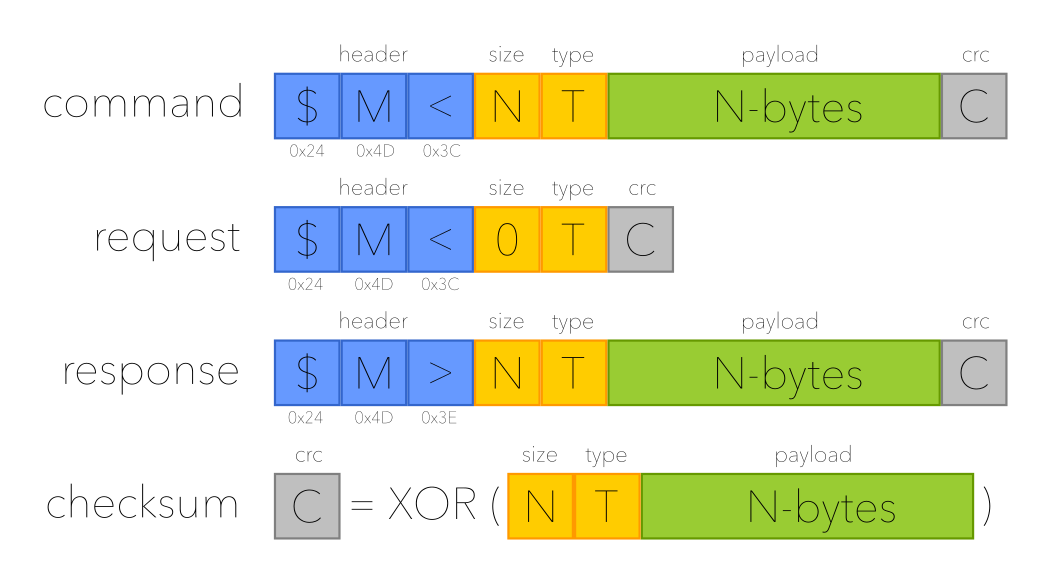
\includegraphics[width=0.9\textwidth]{images/msp_frame}
\caption{MultiWii Serial Protocol (MSP) frame format}
\label{fig:msp}
\end{figure}

\bigskip

In MSP, frames can always be sent to the flight controller (quadcopter). But, in order to receive frames from the flight controller, one has to send a request frame to the flight controller. The request frame is very similar to a command frame, except that its data length is zero and consequently, the checksum is just the MSP message ID.\\

Following is an example to get the attitude and heading data from the flight controller. The MSP message ID for this frame is \textit{108} First we have to send a request frame with an empty payload as follows. The values represented below are decimal ASCII values.\\

\begin{minted}{c}
Request Frame: MSP_ATTITUDE
36 77 60 00 108 108
$  M  <  N  ID  CRC
\end{minted}

\bigskip

\begin{minted}{c}
Response Frame: MSP_ATTITUDE
36 77 62 06 108 6 255 140 0 45 0 50
$  M  >  N  ID  ROLL  PITCH YAW  CRC
\end{minted}

\clearpage

When the size of each data element in the payload is grater than one byte \textit{(UINT8)}, for example, when data types like integers \textit{(INT16)} or long \textit{(UINT32)} are packed in the payload, they are done so starting with LSB first or in little-endian byte order. The payload format for all MSP IDs are given \href{http://www.multiwii.com/wiki/index.php?title=Multiwii_Serial_Protocol}{here}.\\

In the previous example, there are three \textit{INT16} data elements packed as 6 bytes. Another thing to note here, some of the data maybe scaled by a factor (refer to the units \href{http://www.multiwii.com/wiki/index.php?title=Multiwii_Serial_Protocol}{here}) before sending them and must be parsed accordingly. In our example, the data can parsed as follows.\\

\begin{minted}{c}
ROLL = -25 degrees (INT16)
PITCH = 14 degrees (INT16)
HEADING (YAW) = 45 degrees (INT16)
\end{minted}

\bigskip

In the previous example, we requested a frame from the flight controller and got the response. This method is used only to get the data from a flight controller. The next example shows how to send data to the flight controller and update it, like PID gains, throttle and other values. The format remains the same, but the only change here will be the message ID. Following is an example to set the throttle, roll, pitch and yaw controls on the drone. The MSP message ID for this frame is \textit{200}.\\

\begin{minted}{c}
Command Frame: MSP_SET_RAW_RC
36 77 60 16 200 220 05 120 05 220 05 176 04 00 00 00 00 00 00 00 00 17
$  M  <  N  ID  THRO-- ROLL-- PITCH- YAW--- AUX1- AUX2- AUX3- AUX4- CRC$
\end{minted}

\bigskip

On the flight controller, the data can parsed as follows.\\

\begin{minted}{c}
THROTTLE = 1500 (UINT16)
ROLL = 1400 (UINT16)
PITCH = 1500 (UINT16)
YAW = 1200 (UINT16)
AUX1 = 0 (UINT16)
AUX2 = 0 (UINT16)
AUX3 = 0 (UINT16)
AUX4 = 0 (UINT16)
\end{minted}

\section{Implementation in C}
As mentioned earlier, the data payload are stored as structures in memory in C. Following are few examples of different payloads. Note that the header and CRC are not stored and are generated only when required.\\

\begin{minted}{c}
// MSP_ATTITUDE frame - ID: 108
typedef struct __attribute__((__packed__))
{
  int16_t angx;    /* [-1800:1800] 1/10 deg */
  int16_t angy;    /* [-900:900] 1/10 deg */
  int16_t heading; /* [-180:180] deg */
}msp_attitude;
\end{minted}

\bigskip

\begin{minted}{c}
// MSP_SET_RAW_RC frame - ID: 200
typedef struct __attribute__((__packed__))
{
  uint16_t roll;
  uint16_t pitch;
  uint16_t yaw;
  uint16_t throttle;
  uint16_t aux1;
  uint16_t aux2;
  uint16_t aux3;
  uint16_t aux4;
}msp_rc;
\end{minted}

\bigskip
Following is function which takes MSP message ID, the payload and its length as arguments and transmits the frame from the flight controller.\\

\begin{minted}[linenos=true]{c}
void MSP_SendFrame(uint8_t code, uint8_t *data, uint16_t data_length)
{
  uint8_t checksum = 0;

  // Send header $-M->
  serialPrint("$M>");
	
  serialWrite(data_length); // Send data length
  serialWrite(code); // Send code
	
  // Update checksum
  checksum = code ^ data_length;

  // Send data bytes and update checksum
  for (int i=0; i<data_length; i++)
  {
    serialWrite(data[i]);
    checksum ^= data[i];
  }
	
  serialWrite(checksum); // Send checksum
}
\end{minted}

\bigskip

We know that the data payload is stored as a structure. However, in the above snippet, the payload is passed as an byte array to the function. Also, it would be complicated for us to break down the different data elements into bytes and store them into an array. The \textit{memcpy} function \textit{(line 5)} in \textit{string.h} helps us in this process. The following snippet shows how we can transmit the \textit{MSP{\_}RAW{\_}IMU} frame using the previous function. All the structures and message ID macros are defined in \href{./code/msp.h}{\textit{msp.h}}\\

\begin{minted}[linenos=true]{c}
msp_raw_imu msp_txf_raw_imu; // Struct of type msp_raw_imu

void MSP_SendRawIMU()
{
  // Get payload size
  uint16_t data_length = sizeof(msp_raw_imu);				
  
  // Make an empty payload buffer
  uint8_t buff[data_length];	
  
  // Convert struct elements to bytes							
  memcpy(buff, &msp_txf_raw_imu, data_length);
  
  // Pack into MSP frame and transmit		
  MSP_SendFrame(MSP_RAW_IMU, buff, data_length);			
}
\end{minted}

The following is a function to read a MSP frame and just store the data payload into to byte array or buffer.\\

\begin{minted}[linenos=true]{c}
void MSP_Read()
{
  // Buffer to store the payload
  uint8_t buffer[50];
  uint8_t RTS = 0; // Request to send (RTS) flag

  // Check if header matches the sequence $-M-<
  if (serialRead() != '$') return;
  if (serialRead() != 'M') return;
  if (serialRead() != '<') return;
  
  // Read the data length and MSP ID
  uint8_t data_length = serialRead();
  uint8_t code = serialRead();
  
  // Update checksum
  uint8_t checksum = code ^ data_length;
  
  // If data length is non-zero, it is a command frame
  if (data_length != 0)
  {
    for (int i=0; i<data_length; i++)
    {
      // Store data into buffer and update checksum
      buffer[i] = serialRead();
      checksum ^= buffer[i];
    }
  } 
  // If data length is 0, it is a request frame
  else RTS = 1;
  
  // Discard the frame, if checksum doesn't match
  if (checksum != serialRead()) return;
  
  // Parse the frame
  MSP_ParseFrame(code, buffer, data_length, RTS);
}
\end{minted}

The \textit{MSP{\_}ParseFrame} function just consists of a bunch of switch-case statements. If a request frame is received or MSP code is less than 200, the requested frame is sent. If a command frame is received, a callback function is invoked. This callback is declared with \href{http://www.keil.com/support/man/docs/armcc/armcc_chr1359124970859.htm}{\textit{{\_\_}weak}} symbol and the user must implement this function to update the received data, if required. Following is a snippet taken from the \textit{MSP{\_}ParseFrame} function.\\

\begin{minted}[linenos=true]{c}
switch (code)
{
  /* Request frames */

  // Send Raw IMU data on RTS
  case MSP_RAW_IMU:
    if (RTS) MSP_SendRawIMU();													
    break;

  // Send Motor data on RTS
  case MSP_MOTOR:
    if (RTS) MSP_SendMotor();													
    break;
    
  /* Command frames */
  
  case MSP_SET_RAW_RC:
    // Convert byte array to struct
    memcpy(&msp_rxf_raw_rc, data, sizeof(msp_set_raw_rc));
    MSP_SetRawRC_Callback(); // Callback function
    break;

  case MSP_SET_PID:
    // Convert byte array to struct
    memcpy(&msp_rxf_pid, data, sizeof(msp_set_pid));
    MSP_SetPID_Callback(); // Callback function
    break;  
}
\end{minted}

\clearpage

The user must implement the callback function in any other file, but without the {\textit{{\_\_}weak} symbol. For example, the following snippet implements the callback for receiving the motor PWM values sent from a PC.\\

\begin{minted}[linenos=true]{c}
#include "msp.c"

extern msp_set_motor msp_rxf_motor;

void MSP_SetMotor_Callback()
{
  float m1, m2, m3, m4;

  m1 = constrain(msp_rxf_motor.motor[0] - 1000, 0, 1000);
  m2 = constrain(msp_rxf_motor.motor[1] - 1000, 0, 1000);
  m3 = constrain(msp_rxf_motor.motor[2] - 1000, 0, 1000);
  m4 = constrain(msp_rxf_motor.motor[3] - 1000, 0, 1000);

  Motor_SetRawSpeed(m1, m2, m3, m4);
}
\end{minted}

\clearpage

\section{MultiWii Conf Software}
Flight parameters and data like attitude, heading, altitude, motor PWM values, raw IMU data, PID gains and several other data can be visualized in \href{https://code.google.com/archive/p/multiwii/}{MultiWii Conf}, which is open source software written in \textit{Processing}. This software can be used to send or receive data using MSP over a COM port. A virtual COM port can be created with the help of softwares such as \href{https://www.eltima.com/products/serial-over-ethernet/}{Eltima Serial to Ethernet Connector} or \href{http://www.hw-group.com/products/hw_vsp/index_en.html}{HW Virtual Serial Port} which redirects the data from TCP/IP sockets to the COM ports. This can be useful to use MSP over Wi-Fi as well. This is the \href{https://youtu.be/W6h0ePuQfjE}{link} for the video demonstration of the same.\\

\begin{figure}[!htb]
\centering
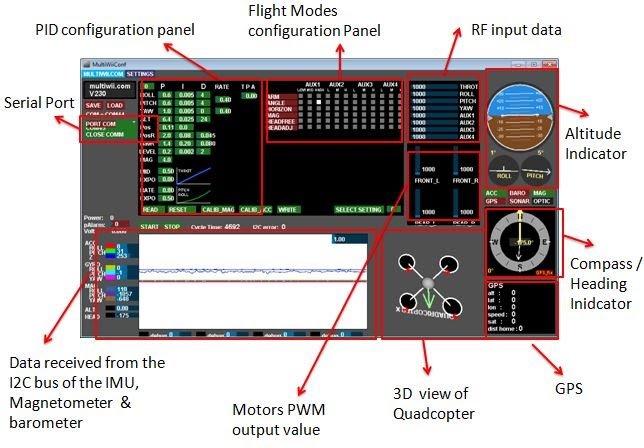
\includegraphics[width=\textwidth]{images/msp_gui}
\caption{MultiWii Conf Software}
\end{figure}

%-------------------------------------------------------------------

\end{document}

